\documentclass[14pt]{beamer}
\usefonttheme[onlymath]{serif}
\usepackage[T2A]{fontenc}
\usepackage[utf8]{inputenc}
\usepackage[english,russian]{babel}
\usepackage{amssymb,amsfonts,amsmath,mathtext}
\usepackage{cite,enumerate,float,indentfirst}

\graphicspath{{Images/}}

\usetheme{Pittsburgh}
\usecolortheme{whale}

\setbeamercolor{footline}{fg=blue}
\setbeamertemplate{footline}{
  \leavevmode%
  \hbox{%
  \begin{beamercolorbox}[wd=.333333\paperwidth,ht=2.25ex,dp=1ex,center]{}%
     Л.\,И. Высоцкий
  \end{beamercolorbox}%
  \begin{beamercolorbox}[wd=.333333\paperwidth,ht=2.25ex,dp=1ex,center]{}%
    Москва, 2018
  \end{beamercolorbox}%
  \begin{beamercolorbox}[wd=.333333\paperwidth,ht=2.25ex,dp=1ex,right]{}%
  Стр. \insertframenumber{} из \inserttotalframenumber \hspace*{2ex}
  \end{beamercolorbox}}%
  \vskip0pt%
}

\newcommand{\itemi}{\item[\checkmark]}

\title{Исследование маятника с осциллирующим подвесом (маятника Капицы)}
\author{Л.И.Высоцкий\vspace{2.5cm}}

\date{\small{Москва, 2018}}

\begin{document}

\maketitle

\begin{frame}
\frametitle{Модель маятника Капицы}
Рассматривается физический маятник с лёгкой нерастяжимой спицей длины $\ell$, прикреплённой одним концом к
подвижной точке подвеса, совершающей вертикальные колебания по закону $y = a \sin(\omega t)$.
\end{frame}

\begin{frame}
\frametitle{Модель маятника Капицы}
\begin{figure}
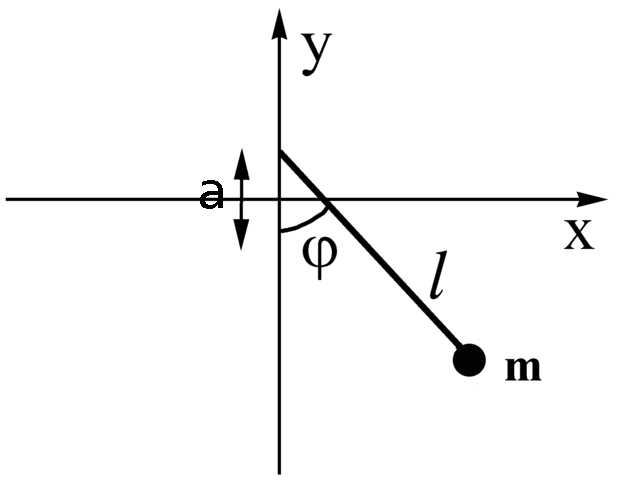
\includegraphics[width=0.6\linewidth]{640px-KapitzaPendulumScheme}
\end{figure}
\pause
Система параметризуется одной обобщённой координатой $\varphi$ -- углом отклонения спицы от вертикали.
\end{frame}


\begin{frame}
\frametitle{Отступление: механика Лагранжа}
\begin{itemize}[<+->]
\item В ньютоновской механике всем рулит 2-ой закон Ньютона $F = m\ddot{r}$.
\item Зная начальные условия (положение и скорость) всех материальных точек системы, а также силы взаимодействия, можно найти положение и скорость в любой момент времени.
\item Однако это не всегда удобно!
\end{itemize}
\end{frame}

\begin{frame}
\frametitle{Отступление: механика Лагранжа}
\begin{itemize}[<+->]
\item Жозеф Луи Лагранж в 1788 предложил свою переформулировку законов классической механики.
\item Система характеризуется обобщёнными координатами $q$. Это могут быть как обычные координаты $x,y,z$, так и любые другие числа, в каждый момент времени полностью описывающие конфигурацию системы.
\end{itemize}
\end{frame}

\begin{frame}
\frametitle{Обобщённые координаты}
\begin{itemize}[<+->]
\item Плоский маятник на жёсткой спице с жёстко закреплённым подвесом --- одна степень свободы и одна обобщённая координата: угол отклонения от вертикали.
\item Маятник Фуко --- две обобщённые координаты: угол поворота плоскости колебаний и угол отклонения маятника от вертикали.
\end{itemize}
\end{frame}

\begin{frame}
\frametitle{Отступление: механика Лагранжа}
\begin{itemize}[<+->]
\item Системе сопоставляется \emph{Лагранжиан} --- функция $L(q,\dot{q},t)$, обычно это $E_K - E_P$
\item \emph{Действие} $S$ --- это интеграл Лагранжиана вдоль заданной траектории:
\[
	S = \int_{t_0}^{t_1}L(q,\dot{q},t)dt.
\]
\item \emph{Принцип наименьшего действия} --- система движется по траектории, соответствующей стационарному действию (концы $(q_0,t_0)$ и $(q_1, t_1)$ фиксированы).
\end{itemize}
\end{frame}

\begin{frame}
\frametitle{Отступление: механика Лагранжа}
\begin{itemize}[<+->]
\item \emph{Принцип наименьшего действия} --- система движется по траектории, соответствующей стационарному действию (концы $(q_0,t_0)$ и $(q_1, t_1)$ фиксированы).
\item Отсюда можно выводить все законы классической механики и, что интереснее, \emph{уравнение Эйлера--Лагранжа}:
\[
\frac{\partial L}{\partial q_i} = \frac{d}{dt}\frac{\partial L}{\partial \dot{q}_i}
\]
\end{itemize}
\end{frame}

\begin{frame}
\frametitle{Уравнение для маятника Капицы}
\begin{itemize}[<+->]
\item Запишем кинетическую и потенциальную энергию системы через $\varphi$, $\dot{\varphi}$ и $t$.
$$
E_K = \frac{m}{2}\left([\ell\cos\varphi\dot{\varphi}]^2 + [\ell\sin\varphi\dot{\varphi} + \omega a \cos(\omega t)]^2\right),
$$
$$
E_P = mg(-\ell\cos\varphi + a\cos(\omega t)).
$$
\item Уравнение Эйлера--Лагранжа (после упрощения):
\[
\ddot{\varphi} = \frac{\sin\varphi}{\ell}(\omega^2a\sin(\omega t) - g).
\]
\end{itemize}
\end{frame}

\begin{frame}
\frametitle{Численное моделирование}
\begin{itemize}[<+->]
\item Запишем в более удобной для численного решения форме:
\[
\begin{cases}
\dot{\varphi} = \psi \\
\dot{\psi} = \frac{\sin\varphi}{\ell}(\omega^2a\sin(\omega t + \gamma) - g) 
\end{cases}
\]
\item Далее будем применять метод Рунге-Кутты 4-го порядка.
\end{itemize}
\end{frame}

\begin{frame}
\begin{center}
\LARGE{Смотрим вживую!}
\end{center}
\end{frame}

\begin{frame}
\frametitle{Устойчивость в вертикальном положении}
\begin{itemize}[<+->]
\item Мы видели, что маятник бывает устойчив в вертикальном положении.
\item Зададим сетку по частоте колебаний подвеса и начальной скорости маятника.
\item Для каждой пары $(\omega, \dot{\varphi}_0)$ промоделируем маятник в течении 50 секунд.
\end{itemize}
\end{frame}

\begin{frame}
\frametitle{Устойчивость в вертикальном положении}
\begin{figure}
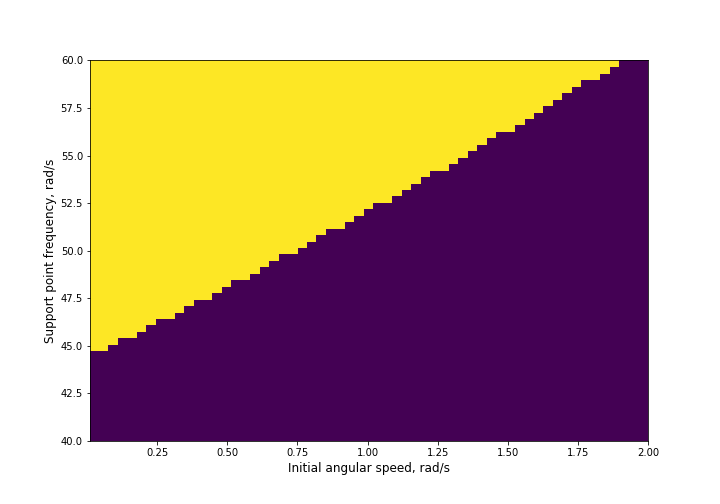
\includegraphics[width=0.9\linewidth]{stabilization.png}
\end{figure}
\end{frame}

\begin{frame}
\begin{center}
\LARGE{Вопросы?}
\end{center}
\end{frame}

\begin{frame}
\begin{center}
\LARGE{Спасибо за внимание!}
\end{center}
\end{frame}

\end{document} 